% Options for packages loaded elsewhere
\PassOptionsToPackage{unicode}{hyperref}
\PassOptionsToPackage{hyphens}{url}
\PassOptionsToPackage{dvipsnames,svgnames,x11names}{xcolor}
%
\documentclass[
  letterpaper,
  DIV=11,
  numbers=noendperiod]{scrartcl}

\usepackage{amsmath,amssymb}
\usepackage{iftex}
\ifPDFTeX
  \usepackage[T1]{fontenc}
  \usepackage[utf8]{inputenc}
  \usepackage{textcomp} % provide euro and other symbols
\else % if luatex or xetex
  \usepackage{unicode-math}
  \defaultfontfeatures{Scale=MatchLowercase}
  \defaultfontfeatures[\rmfamily]{Ligatures=TeX,Scale=1}
\fi
\usepackage{lmodern}
\ifPDFTeX\else  
    % xetex/luatex font selection
\fi
% Use upquote if available, for straight quotes in verbatim environments
\IfFileExists{upquote.sty}{\usepackage{upquote}}{}
\IfFileExists{microtype.sty}{% use microtype if available
  \usepackage[]{microtype}
  \UseMicrotypeSet[protrusion]{basicmath} % disable protrusion for tt fonts
}{}
\makeatletter
\@ifundefined{KOMAClassName}{% if non-KOMA class
  \IfFileExists{parskip.sty}{%
    \usepackage{parskip}
  }{% else
    \setlength{\parindent}{0pt}
    \setlength{\parskip}{6pt plus 2pt minus 1pt}}
}{% if KOMA class
  \KOMAoptions{parskip=half}}
\makeatother
\usepackage{xcolor}
\setlength{\emergencystretch}{3em} % prevent overfull lines
\setcounter{secnumdepth}{-\maxdimen} % remove section numbering
% Make \paragraph and \subparagraph free-standing
\makeatletter
\ifx\paragraph\undefined\else
  \let\oldparagraph\paragraph
  \renewcommand{\paragraph}{
    \@ifstar
      \xxxParagraphStar
      \xxxParagraphNoStar
  }
  \newcommand{\xxxParagraphStar}[1]{\oldparagraph*{#1}\mbox{}}
  \newcommand{\xxxParagraphNoStar}[1]{\oldparagraph{#1}\mbox{}}
\fi
\ifx\subparagraph\undefined\else
  \let\oldsubparagraph\subparagraph
  \renewcommand{\subparagraph}{
    \@ifstar
      \xxxSubParagraphStar
      \xxxSubParagraphNoStar
  }
  \newcommand{\xxxSubParagraphStar}[1]{\oldsubparagraph*{#1}\mbox{}}
  \newcommand{\xxxSubParagraphNoStar}[1]{\oldsubparagraph{#1}\mbox{}}
\fi
\makeatother

\usepackage{color}
\usepackage{fancyvrb}
\newcommand{\VerbBar}{|}
\newcommand{\VERB}{\Verb[commandchars=\\\{\}]}
\DefineVerbatimEnvironment{Highlighting}{Verbatim}{commandchars=\\\{\}}
% Add ',fontsize=\small' for more characters per line
\newenvironment{Shaded}{}{}
\newcommand{\AlertTok}[1]{\textcolor[rgb]{1.00,0.00,0.00}{\textbf{#1}}}
\newcommand{\AnnotationTok}[1]{\textcolor[rgb]{0.38,0.63,0.69}{\textbf{\textit{#1}}}}
\newcommand{\AttributeTok}[1]{\textcolor[rgb]{0.49,0.56,0.16}{#1}}
\newcommand{\BaseNTok}[1]{\textcolor[rgb]{0.25,0.63,0.44}{#1}}
\newcommand{\BuiltInTok}[1]{\textcolor[rgb]{0.00,0.50,0.00}{#1}}
\newcommand{\CharTok}[1]{\textcolor[rgb]{0.25,0.44,0.63}{#1}}
\newcommand{\CommentTok}[1]{\textcolor[rgb]{0.38,0.63,0.69}{\textit{#1}}}
\newcommand{\CommentVarTok}[1]{\textcolor[rgb]{0.38,0.63,0.69}{\textbf{\textit{#1}}}}
\newcommand{\ConstantTok}[1]{\textcolor[rgb]{0.53,0.00,0.00}{#1}}
\newcommand{\ControlFlowTok}[1]{\textcolor[rgb]{0.00,0.44,0.13}{\textbf{#1}}}
\newcommand{\DataTypeTok}[1]{\textcolor[rgb]{0.56,0.13,0.00}{#1}}
\newcommand{\DecValTok}[1]{\textcolor[rgb]{0.25,0.63,0.44}{#1}}
\newcommand{\DocumentationTok}[1]{\textcolor[rgb]{0.73,0.13,0.13}{\textit{#1}}}
\newcommand{\ErrorTok}[1]{\textcolor[rgb]{1.00,0.00,0.00}{\textbf{#1}}}
\newcommand{\ExtensionTok}[1]{#1}
\newcommand{\FloatTok}[1]{\textcolor[rgb]{0.25,0.63,0.44}{#1}}
\newcommand{\FunctionTok}[1]{\textcolor[rgb]{0.02,0.16,0.49}{#1}}
\newcommand{\ImportTok}[1]{\textcolor[rgb]{0.00,0.50,0.00}{\textbf{#1}}}
\newcommand{\InformationTok}[1]{\textcolor[rgb]{0.38,0.63,0.69}{\textbf{\textit{#1}}}}
\newcommand{\KeywordTok}[1]{\textcolor[rgb]{0.00,0.44,0.13}{\textbf{#1}}}
\newcommand{\NormalTok}[1]{#1}
\newcommand{\OperatorTok}[1]{\textcolor[rgb]{0.40,0.40,0.40}{#1}}
\newcommand{\OtherTok}[1]{\textcolor[rgb]{0.00,0.44,0.13}{#1}}
\newcommand{\PreprocessorTok}[1]{\textcolor[rgb]{0.74,0.48,0.00}{#1}}
\newcommand{\RegionMarkerTok}[1]{#1}
\newcommand{\SpecialCharTok}[1]{\textcolor[rgb]{0.25,0.44,0.63}{#1}}
\newcommand{\SpecialStringTok}[1]{\textcolor[rgb]{0.73,0.40,0.53}{#1}}
\newcommand{\StringTok}[1]{\textcolor[rgb]{0.25,0.44,0.63}{#1}}
\newcommand{\VariableTok}[1]{\textcolor[rgb]{0.10,0.09,0.49}{#1}}
\newcommand{\VerbatimStringTok}[1]{\textcolor[rgb]{0.25,0.44,0.63}{#1}}
\newcommand{\WarningTok}[1]{\textcolor[rgb]{0.38,0.63,0.69}{\textbf{\textit{#1}}}}

\providecommand{\tightlist}{%
  \setlength{\itemsep}{0pt}\setlength{\parskip}{0pt}}\usepackage{longtable,booktabs,array}
\usepackage{calc} % for calculating minipage widths
% Correct order of tables after \paragraph or \subparagraph
\usepackage{etoolbox}
\makeatletter
\patchcmd\longtable{\par}{\if@noskipsec\mbox{}\fi\par}{}{}
\makeatother
% Allow footnotes in longtable head/foot
\IfFileExists{footnotehyper.sty}{\usepackage{footnotehyper}}{\usepackage{footnote}}
\makesavenoteenv{longtable}
\usepackage{graphicx}
\makeatletter
\newsavebox\pandoc@box
\newcommand*\pandocbounded[1]{% scales image to fit in text height/width
  \sbox\pandoc@box{#1}%
  \Gscale@div\@tempa{\textheight}{\dimexpr\ht\pandoc@box+\dp\pandoc@box\relax}%
  \Gscale@div\@tempb{\linewidth}{\wd\pandoc@box}%
  \ifdim\@tempb\p@<\@tempa\p@\let\@tempa\@tempb\fi% select the smaller of both
  \ifdim\@tempa\p@<\p@\scalebox{\@tempa}{\usebox\pandoc@box}%
  \else\usebox{\pandoc@box}%
  \fi%
}
% Set default figure placement to htbp
\def\fps@figure{htbp}
\makeatother

\usepackage{fvextra}
\DefineVerbatimEnvironment{Highlighting}{Verbatim}{breaklines=true,breakanywhere=true,commandchars=\\\{\}}
\KOMAoption{captions}{tableheading}
\makeatletter
\@ifpackageloaded{caption}{}{\usepackage{caption}}
\AtBeginDocument{%
\ifdefined\contentsname
  \renewcommand*\contentsname{Table of contents}
\else
  \newcommand\contentsname{Table of contents}
\fi
\ifdefined\listfigurename
  \renewcommand*\listfigurename{List of Figures}
\else
  \newcommand\listfigurename{List of Figures}
\fi
\ifdefined\listtablename
  \renewcommand*\listtablename{List of Tables}
\else
  \newcommand\listtablename{List of Tables}
\fi
\ifdefined\figurename
  \renewcommand*\figurename{Figure}
\else
  \newcommand\figurename{Figure}
\fi
\ifdefined\tablename
  \renewcommand*\tablename{Table}
\else
  \newcommand\tablename{Table}
\fi
}
\@ifpackageloaded{float}{}{\usepackage{float}}
\floatstyle{ruled}
\@ifundefined{c@chapter}{\newfloat{codelisting}{h}{lop}}{\newfloat{codelisting}{h}{lop}[chapter]}
\floatname{codelisting}{Listing}
\newcommand*\listoflistings{\listof{codelisting}{List of Listings}}
\makeatother
\makeatletter
\makeatother
\makeatletter
\@ifpackageloaded{caption}{}{\usepackage{caption}}
\@ifpackageloaded{subcaption}{}{\usepackage{subcaption}}
\makeatother

\usepackage{bookmark}

\IfFileExists{xurl.sty}{\usepackage{xurl}}{} % add URL line breaks if available
\urlstyle{same} % disable monospaced font for URLs
\hypersetup{
  pdftitle={Régression Logistique Binomiale - One-Versus-All (OVA)},
  colorlinks=true,
  linkcolor={blue},
  filecolor={Maroon},
  citecolor={Blue},
  urlcolor={Blue},
  pdfcreator={LaTeX via pandoc}}


\title{Régression Logistique Binomiale - One-Versus-All (OVA)}
\author{}
\date{}

\begin{document}
\maketitle


\subsection{Théorie}\label{thuxe9orie}

La \textbf{régression logistique binomiale} est utilisée pour la
classification binaire, mais elle peut être adaptée aux problèmes
\textbf{multiclasse} via l'approche \textbf{One-Versus-All (OVA)}. Ici,
un modèle est entraîné pour chaque classe contre toutes les autres
combinées.

\subsection{Hyperparamètre utilisé}\label{hyperparamuxe8tre-utilisuxe9}

Nous allons optimiser :

\begin{itemize}
\tightlist
\item
  \textbf{Paramètre de régularisation (\texttt{C})} : qui contrôle la
  complexité du modèle et est sélectionné en fonction de la précision
  sur l'ensemble de validation.
\end{itemize}

\subsection{Métriques d'évaluation}\label{muxe9triques-duxe9valuation}

Nous afficherons :

\begin{itemize}
\item
  \textbf{Matrice de confusion} : montrant les erreurs de classification
  sur l'échantillon de test.
\item
  \textbf{Taux de bien classés sur l'échantillon de validation} avec le
  meilleur hyperparamètre.
\item
  \textbf{Taux de bien classés sur l'échantillon de test} avec ce même
  hyperparamètre.
\item
  \textbf{Taux de bien classés par classe sur l'échantillon de test}
  pour observer la précision sur chaque classe.
\end{itemize}

\subsection{\texorpdfstring{Recherche du meilleur \texttt{C} et
évaluation}{Recherche du meilleur C et évaluation}}\label{recherche-du-meilleur-c-et-uxe9valuation}

\begin{Shaded}
\begin{Highlighting}[]
\ImportTok{import}\NormalTok{ pandas }\ImportTok{as}\NormalTok{ pd}
\ImportTok{import}\NormalTok{ numpy }\ImportTok{as}\NormalTok{ np}
\ImportTok{import}\NormalTok{ matplotlib.pyplot }\ImportTok{as}\NormalTok{ plt}
\ImportTok{from}\NormalTok{ sklearn.linear\_model }\ImportTok{import}\NormalTok{ LogisticRegression}
\ImportTok{from}\NormalTok{ sklearn.multiclass }\ImportTok{import}\NormalTok{ OneVsRestClassifier}
\ImportTok{from}\NormalTok{ sklearn.metrics }\ImportTok{import}\NormalTok{ confusion\_matrix, accuracy\_score}
\ImportTok{from}\NormalTok{ sklearn.preprocessing }\ImportTok{import}\NormalTok{ StandardScaler}
\ImportTok{import}\NormalTok{ warnings}

\CommentTok{\# 🔇 Suppression des avertissements inutiles}
\NormalTok{warnings.filterwarnings(}\StringTok{"ignore"}\NormalTok{, category}\OperatorTok{=}\PreprocessorTok{UserWarning}\NormalTok{)}

\CommentTok{\# 🔄 Chargement des ensembles de données}
\NormalTok{train\_data }\OperatorTok{=}\NormalTok{ pd.read\_csv(}\StringTok{\textquotesingle{}covertype\_train.csv\textquotesingle{}}\NormalTok{)}
\NormalTok{val\_data }\OperatorTok{=}\NormalTok{ pd.read\_csv(}\StringTok{\textquotesingle{}covertype\_val.csv\textquotesingle{}}\NormalTok{)}
\NormalTok{test\_data }\OperatorTok{=}\NormalTok{ pd.read\_csv(}\StringTok{\textquotesingle{}covertype\_test.csv\textquotesingle{}}\NormalTok{)}

\CommentTok{\# 📊 Préparation des données}
\NormalTok{X\_train, y\_train }\OperatorTok{=}\NormalTok{ train\_data.drop(}\StringTok{\textquotesingle{}Cover\_Type\textquotesingle{}}\NormalTok{, axis}\OperatorTok{=}\DecValTok{1}\NormalTok{), train\_data[}\StringTok{\textquotesingle{}Cover\_Type\textquotesingle{}}\NormalTok{]}
\NormalTok{X\_val, y\_val }\OperatorTok{=}\NormalTok{ val\_data.drop(}\StringTok{\textquotesingle{}Cover\_Type\textquotesingle{}}\NormalTok{, axis}\OperatorTok{=}\DecValTok{1}\NormalTok{), val\_data[}\StringTok{\textquotesingle{}Cover\_Type\textquotesingle{}}\NormalTok{]}
\NormalTok{X\_test, y\_test }\OperatorTok{=}\NormalTok{ test\_data.drop(}\StringTok{\textquotesingle{}Cover\_Type\textquotesingle{}}\NormalTok{, axis}\OperatorTok{=}\DecValTok{1}\NormalTok{), test\_data[}\StringTok{\textquotesingle{}Cover\_Type\textquotesingle{}}\NormalTok{]}

\CommentTok{\# 🔢 Normalisation des données}
\NormalTok{scaler }\OperatorTok{=}\NormalTok{ StandardScaler()}
\NormalTok{X\_train, X\_val, X\_test }\OperatorTok{=}\NormalTok{ scaler.fit\_transform(X\_train), scaler.transform(X\_val), scaler.transform(X\_test)}

\CommentTok{\# 🎯 Recherche du meilleur hyperparamètre C}
\NormalTok{C\_values }\OperatorTok{=}\NormalTok{ np.arange(}\FloatTok{0.1}\NormalTok{, }\FloatTok{1.1}\NormalTok{, }\FloatTok{0.1}\NormalTok{)}
\NormalTok{val\_accuracies }\OperatorTok{=}\NormalTok{ []}

\ControlFlowTok{for}\NormalTok{ C }\KeywordTok{in}\NormalTok{ C\_values:}
\NormalTok{    model }\OperatorTok{=}\NormalTok{ OneVsRestClassifier(LogisticRegression(solver}\OperatorTok{=}\StringTok{\textquotesingle{}saga\textquotesingle{}}\NormalTok{, C}\OperatorTok{=}\NormalTok{C, penalty}\OperatorTok{=}\StringTok{\textquotesingle{}l2\textquotesingle{}}\NormalTok{, max\_iter}\OperatorTok{=}\DecValTok{500}\NormalTok{))}
\NormalTok{    model.fit(X\_train, y\_train)}
\NormalTok{    acc }\OperatorTok{=}\NormalTok{ accuracy\_score(y\_val, model.predict(X\_val))}
\NormalTok{    val\_accuracies.append((C, acc))}

\CommentTok{\# Sélection du meilleur hyperparamètre}
\NormalTok{best\_C, best\_val\_acc }\OperatorTok{=} \BuiltInTok{max}\NormalTok{(val\_accuracies, key}\OperatorTok{=}\KeywordTok{lambda}\NormalTok{ x: x[}\DecValTok{1}\NormalTok{])}


\CommentTok{\# 📈 Affichage du graphique}
\NormalTok{plt.figure(figsize}\OperatorTok{=}\NormalTok{(}\DecValTok{8}\NormalTok{, }\DecValTok{6}\NormalTok{))}
\NormalTok{plt.plot(C\_values, [acc }\ControlFlowTok{for}\NormalTok{ C, acc }\KeywordTok{in}\NormalTok{ val\_accuracies], marker}\OperatorTok{=}\StringTok{\textquotesingle{}o\textquotesingle{}}\NormalTok{, linestyle}\OperatorTok{=}\StringTok{\textquotesingle{}dashed\textquotesingle{}}\NormalTok{, label}\OperatorTok{=}\StringTok{"Validation"}\NormalTok{)}
\NormalTok{plt.xlabel(}\StringTok{"Paramètre de régularisation (C)"}\NormalTok{)}
\NormalTok{plt.ylabel(}\StringTok{"Précision sur validation"}\NormalTok{)}
\NormalTok{plt.title(}\StringTok{"Impact de la régularisation sur la performance de la régression logistique (OVA)"}\NormalTok{)}
\NormalTok{plt.legend()}
\NormalTok{plt.show()}

\CommentTok{\# 🏆 Modèle final avec le meilleur hyperparamètre}
\NormalTok{final\_model }\OperatorTok{=}\NormalTok{ OneVsRestClassifier(LogisticRegression(solver}\OperatorTok{=}\StringTok{\textquotesingle{}saga\textquotesingle{}}\NormalTok{, C}\OperatorTok{=}\NormalTok{best\_C, penalty}\OperatorTok{=}\StringTok{\textquotesingle{}l2\textquotesingle{}}\NormalTok{, max\_iter}\OperatorTok{=}\DecValTok{500}\NormalTok{))}
\NormalTok{final\_model.fit(X\_train, y\_train)}
\NormalTok{y\_test\_pred }\OperatorTok{=}\NormalTok{ final\_model.predict(X\_test)}

\CommentTok{\# 📊 Matrice de confusion}
\NormalTok{conf\_matrix }\OperatorTok{=}\NormalTok{ confusion\_matrix(y\_test, y\_test\_pred)}

\CommentTok{\# 📈 Calcul des taux de bien classés par classe}
\NormalTok{class\_accuracies }\OperatorTok{=}\NormalTok{ conf\_matrix.diagonal() }\OperatorTok{/}\NormalTok{ conf\_matrix.}\BuiltInTok{sum}\NormalTok{(axis}\OperatorTok{=}\DecValTok{1}\NormalTok{)}
\NormalTok{overall\_test\_accuracy }\OperatorTok{=}\NormalTok{ accuracy\_score(y\_test, y\_test\_pred)}

\CommentTok{\# 📝 Affichage des résultats}
\BuiltInTok{print}\NormalTok{(}\SpecialStringTok{f"}\CharTok{\textbackslash{}n}\SpecialStringTok{🔹 Meilleur hyperparamètre C sur l\textquotesingle{}échantillon de validation : }\SpecialCharTok{\{}\NormalTok{best\_C}\SpecialCharTok{:.2f\}}\SpecialStringTok{"}\NormalTok{)}
\BuiltInTok{print}\NormalTok{(}\SpecialStringTok{f"Taux de bien classés sur l\textquotesingle{}échantillon de validation avec cet hyperparamètre : }\SpecialCharTok{\{}\NormalTok{best\_val\_acc}\SpecialCharTok{:.2\%\}}\SpecialStringTok{"}\NormalTok{)}
\BuiltInTok{print}\NormalTok{(}\StringTok{"}\CharTok{\textbackslash{}n}\StringTok{📊 Matrice de confusion sur l\textquotesingle{}échantillon de test, avec le meilleur hyperparamètre :"}\NormalTok{)}
\BuiltInTok{print}\NormalTok{(conf\_matrix)}

\BuiltInTok{print}\NormalTok{(}\StringTok{"}\CharTok{\textbackslash{}n}\StringTok{📈 Taux de bien classés par classe sur l\textquotesingle{}échantillon de test, avec le meilleur hyperparamètre  :"}\NormalTok{)}
\ControlFlowTok{for}\NormalTok{ i, acc }\KeywordTok{in} \BuiltInTok{enumerate}\NormalTok{(class\_accuracies, start}\OperatorTok{=}\DecValTok{1}\NormalTok{):}
    \BuiltInTok{print}\NormalTok{(}\SpecialStringTok{f"Classe }\SpecialCharTok{\{}\NormalTok{i}\SpecialCharTok{\}}\SpecialStringTok{ : }\SpecialCharTok{\{}\NormalTok{acc}\SpecialCharTok{:.2\%\}}\SpecialStringTok{"}\NormalTok{)}

\BuiltInTok{print}\NormalTok{(}\SpecialStringTok{f"}\CharTok{\textbackslash{}n}\SpecialStringTok{🔹 Taux de bien classés sur l\textquotesingle{}échantillon de test avec le meilleur hyperparamètre : }\SpecialCharTok{\{}\NormalTok{overall\_test\_accuracy}\SpecialCharTok{:.2\%\}}\SpecialStringTok{"}\NormalTok{)}
\end{Highlighting}
\end{Shaded}

\pandocbounded{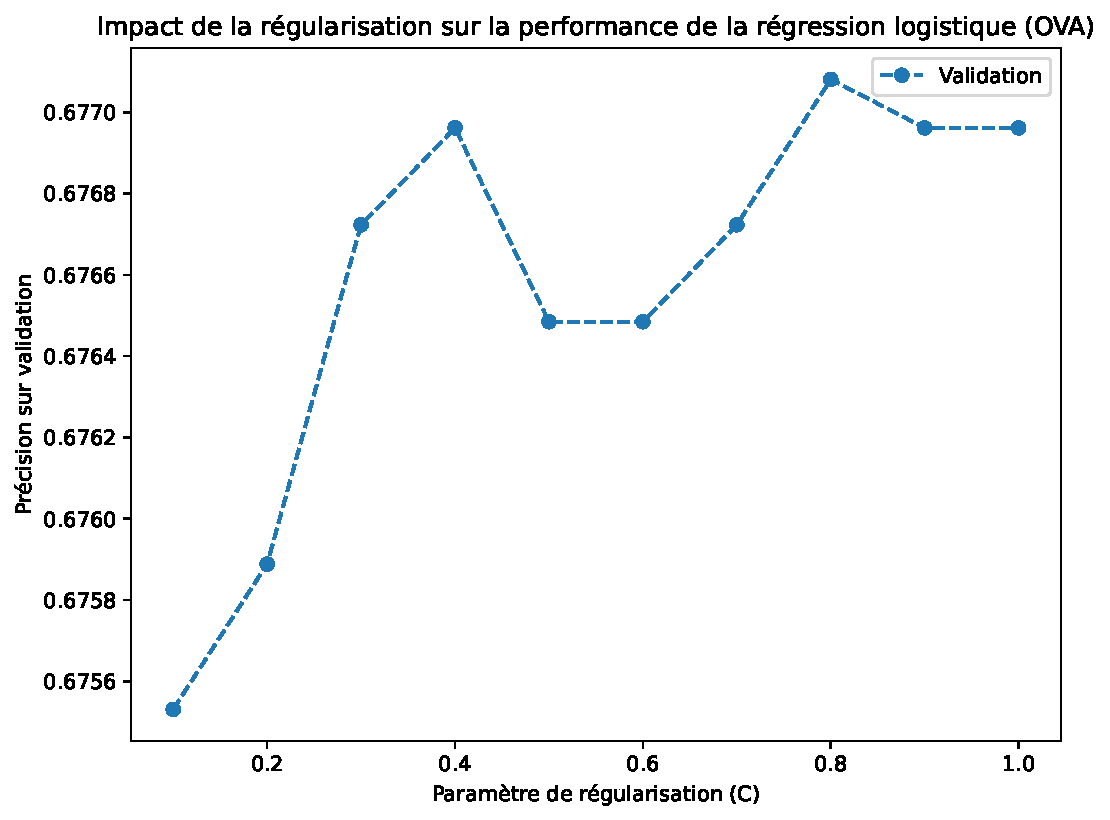
\includegraphics[keepaspectratio]{regression_logistique_ova_files/figure-pdf/cell-2-output-1.pdf}}

\begin{verbatim}

🔹 Meilleur hyperparamètre C sur l'échantillon de validation : 0.80
Taux de bien classés sur l'échantillon de validation avec cet hyperparamètre : 67.71%

📊 Matrice de confusion sur l'échantillon de test, avec le meilleur hyperparamètre :
[[1337  610    1    0    5    1  165]
 [ 495 2150  107    1   21   51    8]
 [   0   65 1270   20    8   67    0]
 [   0    0   70   29    0   11    0]
 [   2  273   27    0   63   15    0]
 [   0   92  386    3   21  192    0]
 [ 143    7    3    0    0    0  668]]

📈 Taux de bien classés par classe sur l'échantillon de test, avec le meilleur hyperparamètre  :
Classe 1 : 63.10%
Classe 2 : 75.89%
Classe 3 : 88.81%
Classe 4 : 26.36%
Classe 5 : 16.58%
Classe 6 : 27.67%
Classe 7 : 81.36%

🔹 Taux de bien classés sur l'échantillon de test avec le meilleur hyperparamètre : 68.07%
\end{verbatim}




\end{document}
